%====================================================================================================
% Monitoramento de servidores Linux por web sites.
%====================================================================================================
% Plano de Trabalho
%----------------------------------------------------------------------------------------------------
% Autor					: Eduardo Balan
% Orientador		: Kleber Kruger
% Instituição 	: UFMS - Universidade Federal do Mato Grosso do Sul
% Unidade				: CPCX - Campus de Coxim
%---------------------------------------------------------------------------------------------------
% Arquivo			: plano_trabalho.tex
% Data de criação	: 29 de Março de 2017
%=====================================================================================================

\chapter{Resultados} \label{cap:Resultados}

Nesta seção são apresentados os resultados do sistema de monitoramento de servidores MonitorWeb. A presente seção é dividida em duas subseções: na \autoref{sec:MonitoreWeb-CliTeste} estão os resultados do MonitorWeb-Cli, e na \autoref{sec:MonitorWeb-ApiTeste} os resultados dos testes do sistema MonitorWeb-Api.


\section{MonitoreWeb-Cli} \label{sec:MonitoreWeb-CliTeste}

Os testes com a aplicação cliente foram executados em diferentes configurações, utilizando-se a ferramenta Valgrind para identificar a existência de vazamentos de memória e de \textit{threads} não liberadas. A primeira sequência de teste descrita na \autoref{subsec:QuantidadeRequisicoesNormais} executou o sistema com uma configuração comum em um ambiente real (monitoramentos de CPU, memória e \textit{swap} sendo realizados em intervalos de 1s). A esta configuração demos o nome de "configuração comum". A segunda sequência de teste, descrita na \autoref{subsec:QuantidadeRequisicoesMaiores} executou o sistema com configuração para um processamento extremo (sem intervalos entre os monitoramentos de CPU, memória e \textit{swap}). A esta configuração demos o nome de "configuração extrema". 

Os testes aplicados nesta seção foram reproduzidos utilizando um computador com processador Intel i5-7200U (2.50GHz a 3.1GHz, cache de 3MB), memória de 8GB (DDR4 2400MHz) e sistema operacional Debian 9 Stretch (Linux Kernel 4.9).

\subsection{Testes com a Configuração Comum} \label{subsec:QuantidadeRequisicoesNormais}

Esse teste teve como objetivo executar todas as operações do sistema cliente verificando o desempenho do processador, memória e \textit{swap}, e detectar eventuais vazamentos de memória (\textit{memory leaks}) em uma situação comum em um ambiente real, em que o monitoramento é realizado a cada segundo. O teste foi repetido 10 vezes, tendo cada teste um tempo de duração de 5 minutos. Esse tempo foi calculado baseando-se em uma duração que fosse suficiente para o atendimento de numerosas requisições, mas dentro de um prazo hábil. As configurações principais do sistema cliente encontra-se na \autoref{Tab:ConfiguraçãoComum}.


\begin{table}[H]
\centering
\label{my-label}
\begin{tabular}{|l|c|}
\hline
\multicolumn{1}{|c|}{{\color[HTML]{000000} \textbf{Configuração}}} & {\color[HTML]{000000} \textbf{Intervalo}} \\ \hline
Envio do registro de monitoramento da CPU                 & 1s                                                                        \\ \hline
Envio do registro de monitoramento da memória             & 1s                                                                        \\ \hline
Envio do registro de monitoramento da \textit{swap}                & 1s                                                                        \\ \hline
Realização da leitura das configurações do servidor       & 5s                                                                       \\ \hline
Envio do registro de monitoramento do PostgreSQL          & 30s                                                                       \\ \hline
Envio do registro de um procedimento de \textit{vacuum}   & 30s                                                                       \\ \hline
Envio do registro de um procedimento de \textit{backup}   & 30s                                                                       \\ \hline
\end{tabular}
\caption[Principais valores da configuração Comum.]{Principais valores da configuração comum.}
\label{Tab:ConfiguraçãoComum}
\end{table}

Os primeiros resultados apresentaram falhas na execução do sistema, pois o Valgrind identificou vazamentos de memória (\textit{memory leaks}) devido a alguns objetos serem alocados dinamicamente e não serem deletados ao final da execução. O mesmo problema ocorreu com as \textit{threads} que eram alocadas estaticamente dentro de um método com escopo local, porém, desacopladas pela função detach. Esta função permite a uma \textit{thread} continuar a execução de forma independente, assim, elas não eram liberadas ao término do programa e geravam vazamentos.

Após algumas refatorações do código o resultado foi satisfatório, isto é, nenhuma das 10 execuções apresentou falhas. Cabe observar que não haver vazamentos de memória é um requisito de suma importância às aplicações, principalmente àquelas que executam por um longo período de tempo, pois vazamentos de memória reduzem a quantidade de memória disponível, e consequentemente, debilita o desempenho do computador.

O relatório apresentado pela ferramenta Valgrind pode ser visto na \autoref{Img:resultado5Valgrind}.


\begin{figure}[H]
	\centering
	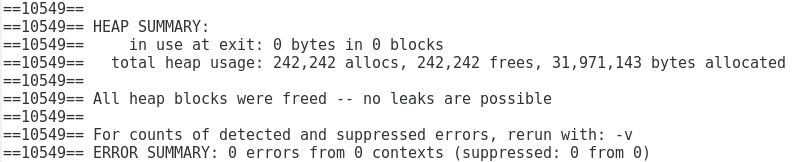
\includegraphics[width=0.8\textwidth]{figuras/monitorWebCliTeste1/resultado5.JPG}
	\caption[Resultado do Valgrind com configuração comum.]{Resultado do Valgrind com configuração comum. Pode ser visto que todas as memórias que foram alocadas pela aplicação foram desalocadas e que zero erros foram encontrados em zero contextos diferentes.}
	\label{Img:resultado5Valgrind}
\end{figure}



Na \autoref{Img:ConsumoDoSistema} pode ser visto o consumo de recursos do \textit{hardware} que a aplicação MonitoreWeb-Cli estava consumindo durante os 5 minutos de execução de um dos testes. Nela pode ser observado o uso do processador (\%CPU) que foi crescendo gradualmente até se estabilizar em 0,5\% tendo uma media de 0,44\% e desvio padrão de 0.09057\%. O mesmo pode ser observado com a memória virtual (VSZ), que foi estabilizada em 906960 (0.864944 Mb). Outro valor a ser observado é o tempo total da CPU utilizada pelo processo desde que foi iniciado (TIME), que ficou em aproximadamente 1 segundo dentro de um período de monitoramento de 5 minutos. A lista a seguir descreve o significado das principais colunas da figura.


%SERIA IDEAL APRESENTAR O CONSUMO MÉDIO. Média (Average)  Média (Average) 0.44,  Desvio padrão 0.09057
% 0.1,0.2,0.2,0.2,0.3,0.3,0.4,0.4,0.4,0.4,0.4,0.4,0.4,0.4,0.5,0.4,0.4,0.4,0.5,0.4,0.4,0.4,0.4,0.4,0.5,0.4,0.4,0.5,0.4,0.5,0.5,0.5,0.5,0.5,0.5,0.5,0.5,0.5,0.5,0.5,0.5,0.5,0.5,0.5,0.5,0.5,0.5,0.5,0.5,0.5,0.5,0.5,0.5,0.5,0.5,0.5,0.5,0.5,0.5,0.5  Média (Average) 0.44,  Desvio padrão 0.09057

\begin{itemize}
    \item PID: número de identificação do processo.
    
    \item \%CPU: consumo de processamento do processo.
    
    \item \%MEM: consumo de memória do processo.
     
    \item VSZ: tamanho da memória virtual, que corresponde à memória do processo mais a memória de bibliotecas compartilhadas.
    
    \item RSS: soma total da memória física usada pelo processo.
    
    \item TIME: tempo total da CPU usado pelo processo desde que foi iniciado.
        
    \item COMMAND: Nome do comando do processo.

\end{itemize}
\begin{figure}[H]
	\centering
	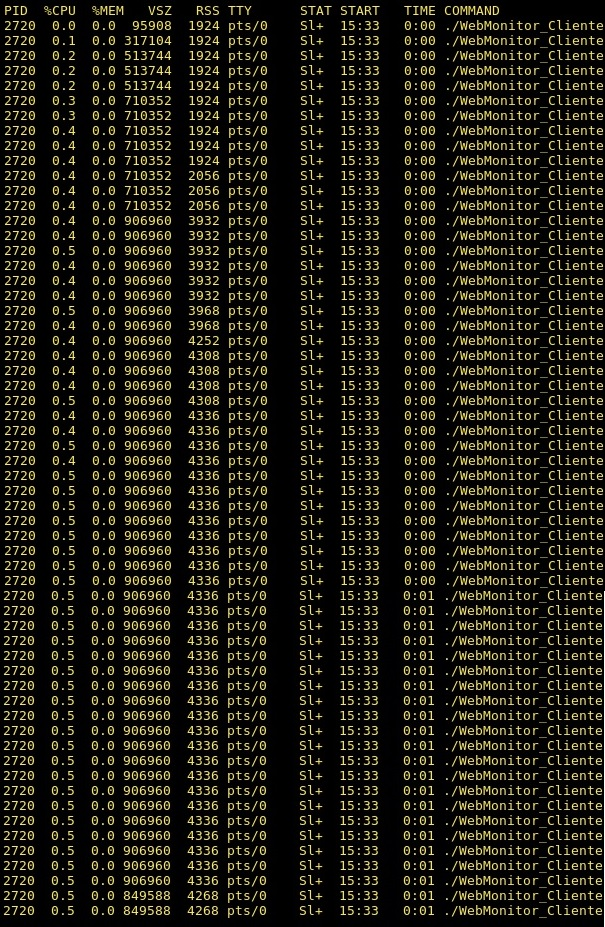
\includegraphics[width=0.8\textwidth]{figuras/monitorWebCliTeste1/hardware.JPG}
	\caption[Consumo de recursos do \textit{hardware} com a configuração comum.]{Consumo de recursos do \textit{hardware} com a configuração comum. A coluna \%CPU representa o consumo de processamento, esse valor foi estabilizado em 0,5\% tendo uma media de 0,44\% e desvio padrão de 0.09057\%.}
	\label{Img:ConsumoDoSistema}
\end{figure}



% # # # # # # # # # # # # # # # # # # # # # # # # # # # # # # # # # # # # # # # # # # # # # # # # # # # # # # # # # # # # # # # # # # # # # # # # # # # # # # # # # # # # # # # # # # # # # # # # # # # # # # # # # # # # # # # # # # # # # # # # # # # # # # # # # # # # # # # # # # # # # # # # # # # # # # # # # # # # # # # # # # # # # # # # # # # # # # # # # # # # # # # # # # # # # # # # # # # # # # # # # # # # # # # # # # # # 

\subsection{Testes com Configuração Extrema} \label{subsec:QuantidadeRequisicoesMaiores}

Esse teste teve como objetivo executar todas as operações do sistema cliente sem intervalos, causando uma situação extrema de processamento, uso de memória e uso do disco. Conforme descrito anteriormente, essa configuração não é recomendada devido ao fato de sobrecarregar a máquina cliente, sem apresentar contraponto relevante, uma vez que o monitoramento a cada 1s é suficiente para um monitoramento preciso. Essa configuração foi utilizada no teste com a intenção de gerar um processamento elevado, aumentando a possibilidade do Valgrid detectar falhas. O teste foi repetido 5 vezes, tendo um tempo de duração de 5 minutos. As configurações principais do sistema cliente encontra-se na \autoref{Tab:ConfiguraçãoExtrema}.


\begin{table}[H]
\centering
\label{my-label}
\begin{tabular}{|l|c|}
\hline
\multicolumn{1}{|c|}{{\color[HTML]{000000} \textbf{Configuração}}} & {\color[HTML]{000000} \textbf{Intervalo}} \\ \hline
Envio do registro de monitoramento da CPU                 & 0s                                                                        \\ \hline
Envio do registro de monitoramento da memória             & 0s                                                                        \\ \hline
Envio do registro de monitoramento da \textit{swap}                & 0s                                                                        \\ \hline
Realização da leitura das configurações do servidor       & 1s                                                                       \\ \hline
Envio do registro de monitoramento do PostgreSQL          & 30s                                                                       \\ \hline
Envio do registro de um procedimento de \textit{vacuum}   & 30s                                                                       \\ \hline
Envio do registro de um procedimento de \textit{backup}   & 30s                                                                       \\ \hline
\end{tabular}
\caption[Principais valores da configuração extrema.]{Principais valores da configuração extrema.}
\label{Tab:ConfiguraçãoExtrema}
\end{table}

O resultado foi satisfatório, nenhuma das 5 execuções do teste apresentaram defeito. O relatório apresentado pela ferramenta Valgrind pode ser visto na \autoref{Img:resultado5Valgrindteste2}.

\begin{figure}[H]
	\centering
	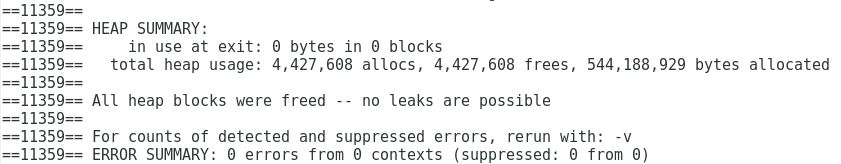
\includegraphics[width=1.0\textwidth]{figuras/monitorWebCliTeste2/resultado5 minutos.jpg}
	\caption[Resultado do Valgrind com processamento extremo.]{Resultado do Valgrind com processamento extremo. Cabe observar que toda a memória alocada pela aplicação foi desalocada, e que zero erros foram encontrados.}
	\label{Img:resultado5Valgrindteste2}
\end{figure}

%SERIA IDEAL APRESENTAR O CONSUMO MÉDIO. Média (Average) 25.99016, Desvio padrão 4.4445
% 3.2,11.1,14.4,16.1,19.3,21.8,22.4,23.1,24.9,25.7,26.4,26.5,26.7,26.7,26.9,27.2,27.3,27.3,27.5,27.5,27.5,27.5,27.5,27.5,27.5,27.5,27.5,27.5,27.5,27.4,27.4,27.2,27.2,27.2,27.3,27.3,27.3,27.4,27.4,27.5,27.5,27.6,27.6,27.7,27.7,27.7,27.7,27.8,27.8,27.9,27.9,27.9,27.9,28,28,28,28,28.1,28.1,28.2,28.2   https://www.easycalculation.com/pt/statistics/standard-deviation.php  Média (Average) 25.99016, Desvio padrão 4.4445

Na \autoref{Img:consumo2} mostra-se o consumo de recursos do \textit{hardware} que a aplicação MonitoreWeb-Cli consumiu durante os 5 minutos da execução de um dos testes. Nela, o uso do processador (\%CPU) foi crescendo gradualmente até se estabilizar em aproximadamente 27,5\% tendo uma média de 25.99016\% e desvio padrão de 4.4445\%. O mesmo pode ser observado com a memória virtual (VSZ), que foi estabilizada em 906960 (0.864944 Mb) - mesmo resultado do teste da \autoref{subsec:QuantidadeRequisicoesNormais}. Outro valor a ser observado é o tempo que o sistema dedicou exclusivamente para a aplicação (TIME), que ficou em aproximadamente 1 minuto e 26 segundos em um período total de monitoramento de 5 minutos.

\begin{figure}[H]
	\centering
	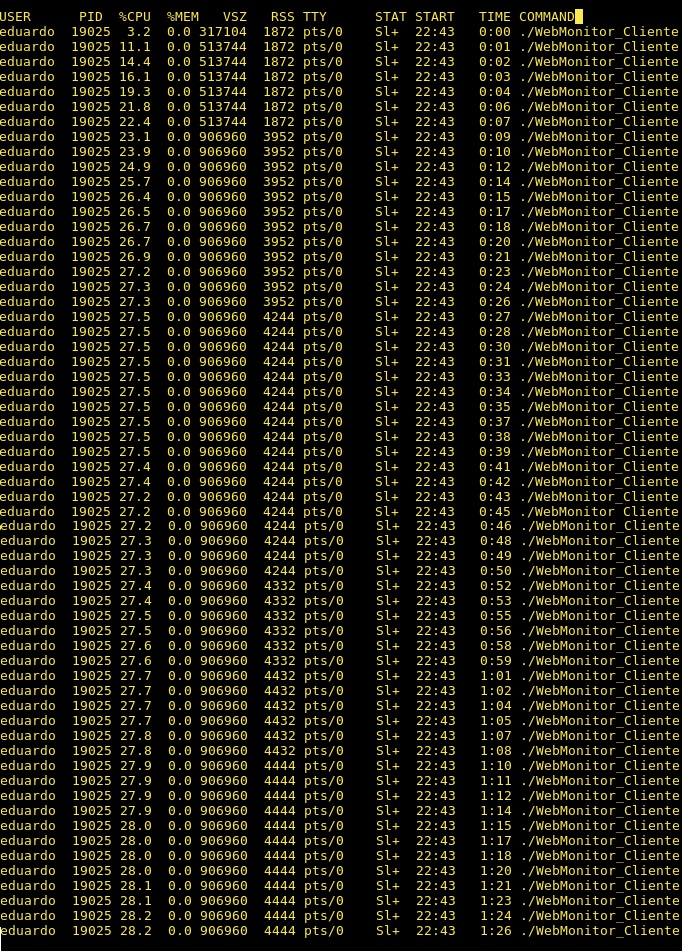
\includegraphics[width=0.8\textwidth]{figuras/monitorWebCliTeste2/hardwareTeste2.jpg}
	\caption[Consumo de recursos do \textit{hardware} com configuraçãos extremas.]{Consumo de recursos do \textit{hardware} com configurações extremas.  A coluna \%CPU representa o consumo de processamento, esse valor foi estabilizado em torno de 27,5\% tendo uma media de 25.99016\% e desvio padrão de 4.4445\%}
	\label{Img:consumo2}
\end{figure}


\section{MonitorWeb-Api} \label{sec:MonitorWeb-ApiTeste}

Nesta seção descreve-se os testes unitários, vistos anteriormente na \autoref{sec:TestesAutomatizados}. Estes, tiveram o intuído de trazer a confiabilidade de que todos os recursos da aplicação funcionam corretamente. Além disso, foi realizado testes para verificar o desempenho (em termos de uso de memória e de CPU, e quantidade de requisições atendidas) do servidor web durante diferentes cargas de requisição.

\subsection{Testes de Unidade}\label{}

Para a realização dos teste de unidade foi utilizado a ferramenta Spring Boot Test, vista na \autoref{subsec:SpringTest}. Todos os teste citados nesta subseção podem ser encontrados no pacote \url{/src/test} do projeto.

Foram realizados testes de unidade para todos os recursos da aplicação. Os testes foram realizados de acordo com a funcionalidade de cada recurso. A \autoref{Img:PlanilhaTesteUnidade} mostra quais testes foram realizados em cada recurso da aplicação.

Os testes descritos na lista a seguir fazem os seguintes procedimentos:

\begin{itemize}
    \item buscarPorIdTest: efetua uma busca por id e verifica se o objeto recebido corresponde ao objeto desejado.
    
    \item buscarTodosTest: efetua uma busca e verifica se todos os objetos do banco de dados foram trazidos com sucesso.
    
    \item buscarTodosPorServidorTest: efetua uma busca por id de um Objeto Servidor e verifica se os valores obtidos são os desejados.
    
    \item buscarIdInexistenteServidorTest: efetua uma busco por id de um Objeto Servidor inexistente e verifica se retorna o valor esperado.
    
    \item deletarTest: deleta um registo e verifica se ele foi realente deletado.
    
    \item deletarIdInexistenteTest: tenta deletar um registro que não existe e verifica se o sistema retorna o valor esperado.
    
    \item inserirTest: insere um registro e verifica se os valores inseridos estão corretos.
\end{itemize}
 

\begin{figure}[H]
	\centering
	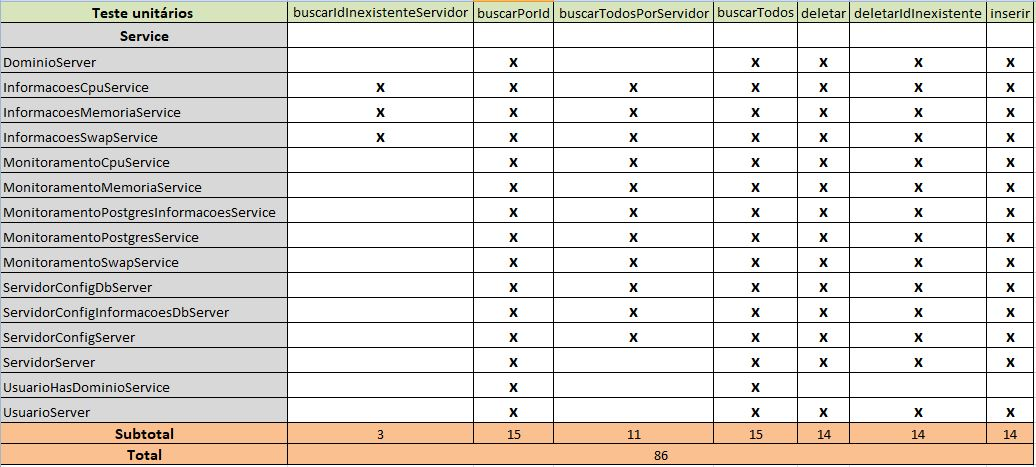
\includegraphics[width=1.0\textwidth]{figuras/MonitorWebApiTeste3/Teste3Planilha.jpg}
	\caption[Planilha de intersecção dos testes de unidade com services]{Planilha de intersecção dos testes de unidade com services, onde a intersecção representada pela letra X indica que o teste foi realizado.}
	\label{Img:PlanilhaTesteUnidade}
\end{figure}


Na \autoref{Img:testeUnitarioOk} pode ser visto todos os 86 testes unitários executados com sucesso.

\begin{figure}[H]
	\centering
	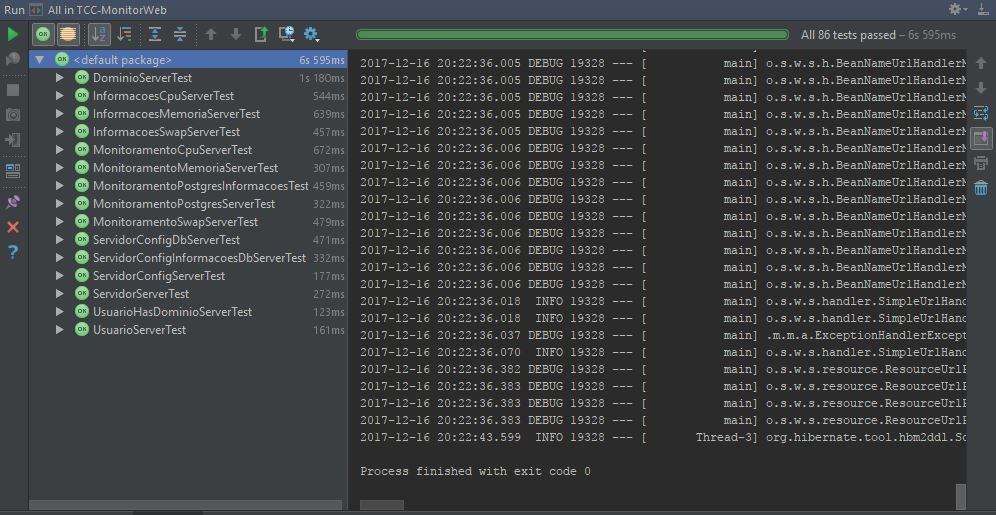
\includegraphics[width=1.0\textwidth]{figuras/MonitorWebApiTeste3/ResultadoTeste2.jpg}
	\caption[IntelliJ executando os 86 testes de unidade com sucesso]{IntelliJ executando os 86 testes de unidade com sucesso}
	\label{Img:testeUnitarioOk}
\end{figure}


\subsection{Teste de Desempenho do MonitorWeb-Api} \label{}

Os teste apresentados nesta seção tem como objetivo medir o desempenho da aplicação MonitorWeb-Api, verificando sua capacidade de monitoramento e consumo de recursos do \textit{hardware}.

Para execução desse teste, foi utilizado dois computadores: um executando a aplicação servidor (MonitorWeb-Api) e outro executando a aplicação cliente (MonitorWeb-Cli).

\begin{itemize}
    \item MonitorWeb-Api: computador com processador Intel i7-4500U (1.80GHz a 3.00GHz, Cache de 4MB), memória de 16GB (DDR3 1600MHz), SDD de 480GB (Modelo SA400S37480G, capacidade de leitura: 500MBs/s, capacidade de gravação: 450MB/s) e sistema operacional Windows 10 Professional.
    
    \item MonitorWeb-Cli: computador com processador Intel i5-7200U (2.50GHz a 3.1GHz, Cache de 3MB), memória de 8GB (DDR4 2400MHz) e sistema operacional Debian 9 Stretch (Linux Kernel 4.9).
\end{itemize}

\subsubsection{Quantidade de consumo com a configuração comum} \label{subsec:APIQuantidadeRequisicoesNormais}

Esse teste teve o objetivo de executar a aplicação MonitorWeb-Api juntamente com o sistema cliente. As configurações utilizadas para o sistema cliente foram as mesmas do teste com as configurações comum mostrado na \autoref{subsec:QuantidadeRequisicoesNormais}.

Na \autoref{Img:BaixoProcessametno} mostra-se dois gráficos: no primeiro apresenta-se o consumo de memória (\textit{memory}) e no segundo apresenta-se consumo de CPU (\textit{CPU Load}), tendo o teste a duração de 8 minutos. Do minuto 0:00 ao 0:16 a aplicação estava sendo iniciada; do 0:16 ao 1:06 ficou em estado de espera por uma aplicação cliente; no minuto 1:07, foi iniciada a comunicação com a aplicação cliente que durou até o minuto 7:00. Após isso, a aplicação cliente terminou.

\begin{figure}[H]
	\centering
	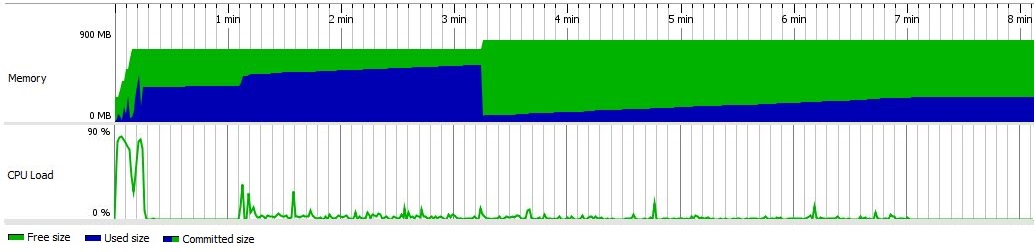
\includegraphics[width=1.0\textwidth]{figuras/MonitorWebApiTeste4/BaixoProcessametno.jpg}
	\caption[Quantidade de consumo com a configuração comum]{Quantidade de consumo do sistema MonitorWeb-Api com a configuração comum. Dois gráficos podem ser vistos na figura. O primeiro representa o consumo de memoria da aplicação servidor e o segundo o consumo de CPU.}
	\label{Img:BaixoProcessametno}
\end{figure}



\subsubsection{Teste com Processamento Extremo}\label{subsec:APIQuantidadeRequisicoesMaior}


Neste teste, as configurações utilizadas para o sistema cliente foram as mesmas da \autoref{subsec:QuantidadeRequisicoesMaiores}, entretanto, não houve intervalo entre as consultas de monitoramento, e dessa forma, pode-se analisar o comportamento das duas aplicações sobre uma carga de processamento extrema.

Na figura \autoref{Img:BaixoProcessametno} apresenta-se dois gráficos: o primeiro sobre o consumo de memória (\textit{memory}) e o segundo sobre consumo de CPU (\textit{CPU Load}) com duração de 9 minutos. Do minuto 0:00 ao 0:16 a aplicação estava sendo iniciada; do 0:16 ao 1:12 a aplicação estava esperando por uma aplicação cliente para iniciar a comunicação; no minuto 1:13 é iniciado a comunicação com a aplicação cliente, que durou até o minuto 8:30. Após isso, a aplicação cliente foi encerrada.

\begin{figure}[H]
	\centering
	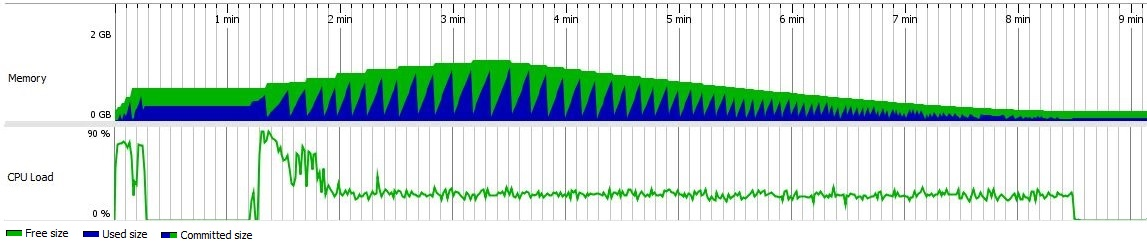
\includegraphics[width=1.0\textwidth]{figuras/MonitorWebApiTeste4/AutoProcessametno.jpg}
	\caption[Quantidade de consumo com a configuração extrema]{Quantidade de consumo do sistema MonitorWeb-Api com a configuração extrema. Dois gráficos podem ser vistos na figura. O primeiro representa o consumo de memoria da aplicação servidor e o segundo o consumo de CPU}
	\label{Img:AutoProcessametno.jpg}
\end{figure}

Na figura \autoref{Img:GerenciadorDoWindows5} e na \autoref{Img:GerenciadorDoWindows5-2.jpg} pode ser observado que o banco de dados PostgreSQL teve grande contribuição para o SSD atingir 100\% de seu desempenho, gerando um gargalo para a aplicação. 

Na figura \autoref{Img:sql1.jpg} mostra-se a quantidade de registros inseridos no banco de dados no intervalo de 7:17 minutos. Neste período, foram inseridos no banco de dados 76911 registros de CPU, 80078 registros de memória e 81762 registros \textit{swap}, o que dá, respectivamente, uma taxa de 175,99/s, 183,24/s, e 187,09/s. Esses valores totalizam em média, a inserção de 546,34 registros por segundos.

\begin{figure}[H]
	\centering
	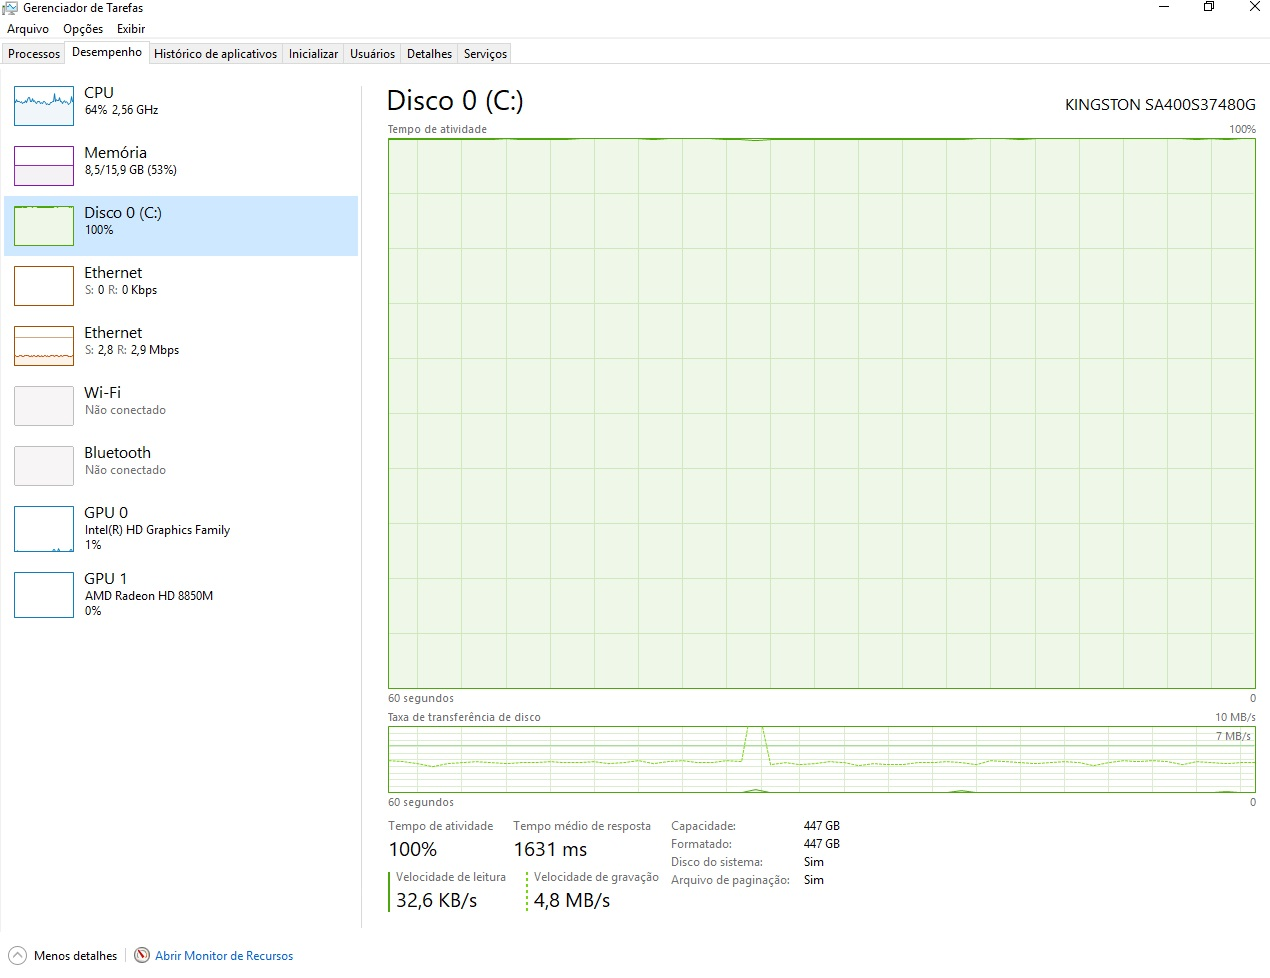
\includegraphics[width=1.0\textwidth]{figuras/MonitorWebApiTeste4/GerenciadorDoWindows5.jpg}
	\caption[Gerenciador de tarefas do Windows mostrando o consumo de recursos]{Gerenciador de tarefas do Windows mostrando o consumo do SSD em 100\%}
	\label{Img:GerenciadorDoWindows5}
\end{figure}

\begin{figure}[H]
	\centering
	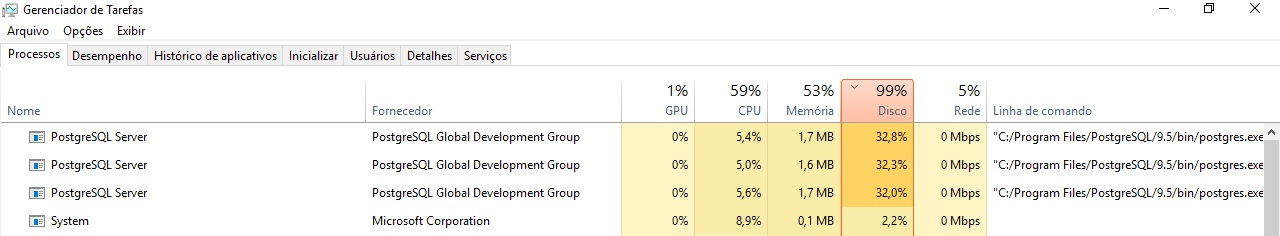
\includegraphics[width=1.0\textwidth]{figuras/MonitorWebApiTeste4/GerenciadorDoWindows5-2.jpg}
	\caption[Gerenciador de tarefas do Windows mostrando os principais processos]{Gerenciador de tarefas do Windows mostrando os principais processos}
	\label{Img:GerenciadorDoWindows5-2.jpg}
\end{figure}

\begin{figure}[H]
	\centering
	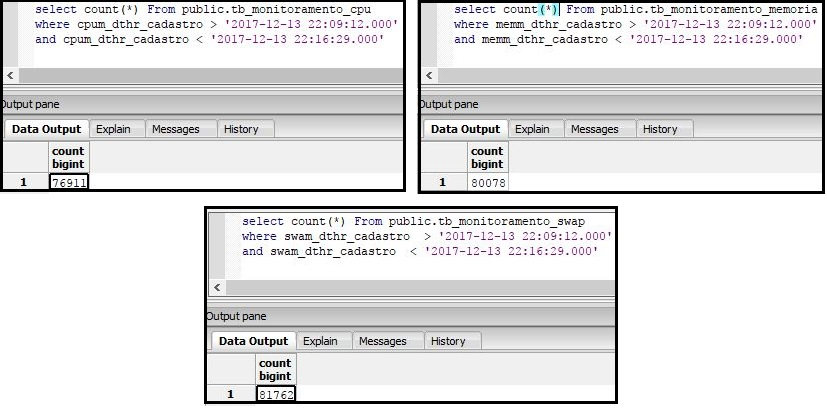
\includegraphics[width=1.0\textwidth]{figuras/MonitorWebApiTeste4/sql1.jpg}
	\caption[Quantidade de registros inseridos no banco de dados.]{Quantidade de registros inseridos no banco de dados no intervalo de 7:17 minutos.}
	\label{Img:sql1.jpg}
\end{figure}
